\clearpage
\subsection{Current live execution and independent validation}
\label{sec:live-validation}
Both final sessions ran on 14 September 2026 UTC (the local Netherlands date
crossed into 15 September during the work). Each captured 180 complete one-second
epochs using one public caster connection. CPU and CUDA ran sequential sessions:
CPU: 21:55:20--21:58:20 UTC; CUDA: 21:58:54--22:01:54 UTC. The source is \code{caster.centipede.fr:2101/LIENSS}.
\begin{center}
\begin{tabularx}{\textwidth}{@{}P{.61\textwidth}YY@{}}\toprule
\textbf{Measured quantity} & \textbf{CPU} & \textbf{CUDA}\\\midrule
Complete received epochs & 180 & 180\\
Published native positions & 172 & 175\\
Initial unavailable epochs (ephemeris warmup) & 8 & 5\\
Initial ECEF/clock seed & Zero & Zero\\
Mean 3D separation from advertised ARP (m) & 1.644 & 1.854\\
Maximum ARP separation (m) & 2.232 & 2.267\\
Mean 3D difference from RTKLIB (m) & 0.649 & 0.622\\
Maximum RTKLIB difference (m) & 0.969 & 0.931\\
Median complete-input-to-position (ms) & 2.205 & 5.947\\
Maximum complete-input-to-position (ms) & 11.611 & 14.346\\
All positions emitted during socket capture & Yes & Yes\\\bottomrule
\end{tabularx}
\end{center}
The native outputs and their timestamps were checked against the exact raw-frame
hashes and receive-chunk sidecars. The latency above runs from the host receiving
the final required input fragment to publication of a valid position. It includes
local decoding and solving; it is not a calibrated radio/network transit time.
It excludes unavailable warmup epochs. CUDA's first unavailable live epoch took
2.59 seconds inside processing, including initial device work. A separate
persistent-worker regression measured about 1.05 seconds for its first request.
CPU is faster for this small 1 Hz workload; these results establish CUDA correctness,
not a speedup. The CUDA device was the RTX 5070 Ti Laptop, compute capability 12.0,
built with CUDA 12.8 and driver 591.59.

The comparison coordinate is the stream's advertised antenna reference point:
\begin{equation}
 (4426043.0455,\ -89429.1998,\ 4576296.6447)\ \mathrm m.
\end{equation}
It was neither a supplied initial estimate nor an observation. It is not an
independently surveyed truth coordinate in this experiment. Consequently the table
reports separation from advertised ARP, not certified absolute accuracy. RTKLIB
also performs single-point code positioning here; its output quality code is 5,
not an RTK fixed-ambiguity solution.

\clearpage
\subsection{Measured position series and independent checks}
\begin{center}
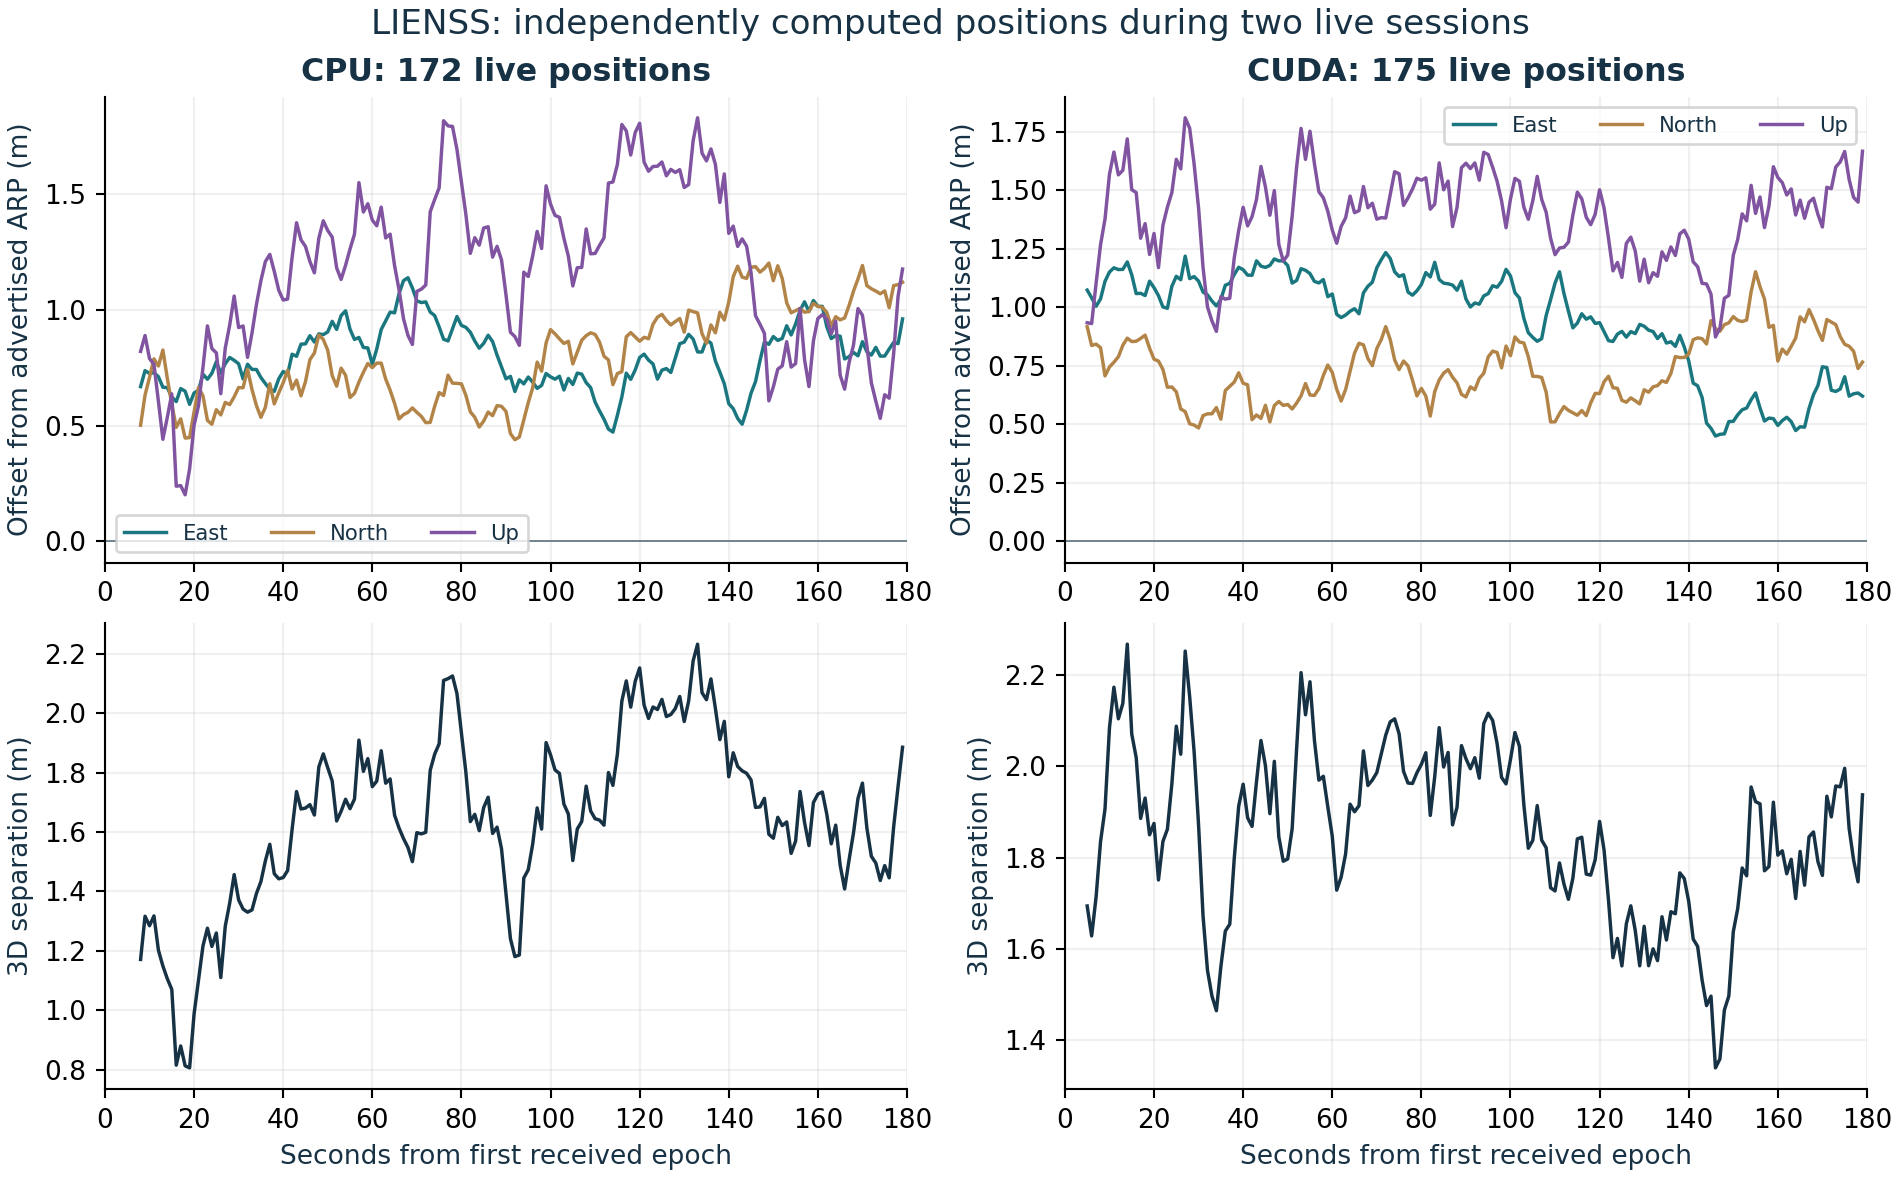
\includegraphics[width=\textwidth]{figures/live_position_evidence.png}
\end{center}
\textbf{Figure.} East/North/Up and three-dimensional separation from the advertised
ARP in the two actual live sessions. The blank beginning is ephemeris warmup;
no position is fabricated for it. These are different time windows, so their
physical differences are not a CPU-versus-GPU numerical comparison.

For that numerical comparison, the same final raw capture was replayed through
both backends with the same preparation model and receive order. Both produced
175 positions from 180 epochs; their maximum ECEF/clock component difference was
$1.21\times10^{-8}$ m. Live CUDA and its archived-byte replay also passed the same
epoch/status/position comparison. \path{results/live_cross_backend.json} records it.

The independent published RTKLIB \code{convbin} decoded each capture to RINEX.
The final CPU and CUDA decoded satellite/epoch sets matched exactly; 1980 and
2094 common C1C ranges agreed to 0.279 mm, within RINEX decimal rounding. Respectively
280 and 588 ephemeris numeric fields agreed. A separate pyrtcm field audit on the
five-minute source capture passed 96,880 comparisons. The orbit/clock oracle
matched eight satellite positions to 0.578 mm and clocks to 0.000438 ns, limited
by its printed output precision. Source hashes and commands are retained.

\clearpage
\subsection{Regression, real-model checks and retained state connection}
The older GSI recording solved all 120 real epochs from ECEF zero. Its raw physical
model and weight-isolation experiment are described with the equations above.
Prepared final live CPU observations passed 3,324 independent Householder checks
across all 180 epochs, with maximum state-component difference below
$8.4\times10^{-9}$ m. All partial/warmup statuses were retained. The persistent
CUDA worker processed those same real final-pass inputs under Compute Sanitizer:
zero memory errors, 180 responses and 1,048 independent checks.

Current native builds passed all three CTest suites on CPU and CUDA. Python passed
118 test methods. The persistent-interface regression passed 6,861 comparisons
per backend, including rejected requests followed by successful recovery.
The existing texture/global CUDA paths also passed independent comparison and
Compute Sanitizer through \code{validate\_gpu.py --sanitizer}. Analytic/parser tests
cover wrong CRC, fragments, missing data, stream truncation, HTTP chunking,
reconnection, callback failure, stale epochs, native failure and cold-start rules.

Independent NumPy re-solves verified all 698 converged outer passes across both
final live sessions to $1.40\times10^{-8}$ m per component. The physical audit
checked 6,284 prepared rows, including original code, correction signs and proof
that every chosen 1019 issue had already arrived before its epoch was solved.
All 347 published fixes preserve the corrected reception-time equation.

The same live position records also cross the retained CGK-R1 handoff after
capture. Only completed positions enter that downstream replay; omitted warmup
epochs remain listed in its manifest. ENU is anchored at the first computed
position, never at the advertised ARP. Original IDs, ECEF, receiver clock and full
time remain attached. Both key layouts are emitted wherever the chart is defined.
The stationary demonstration does not require the word state to switch, and its
modeled mechanics are not interpreted as a measured receiver velocity. The final
CPU bridge retained 172 fixes and listed eight warmup omissions; its native batch
position/clock replay exactly matched the stream. CGK replay passed 16,684 field
comparisons, and a separate binding audit passed 1,042 checks. The word remained
$q=0$ in this static session. Both keys were emitted for 153 positions; 19
remained inside the chart core. These facts do not assert dynamic switching.

\textbf{Evidence index.} \path{results/validation_status.json} links current
reports and their hashes. \path{results/network_probes/} contains the independent
conversion, raw-field and RTKLIB comparisons. \path{source/live_data/README.md}
records data provenance and third-party attribution. Parent 3.6.1.7 totals in
the following chapters are explicitly historical and are not added to these
live-session results. The original sibling release remains unchanged.
